\documentclass[11pt]{utalcaDoc}
\usepackage{alltt}
\usepackage{underscore}
\usepackage[utf8]{inputenc}
\usepackage[activeacute,spanish]{babel}
\usepackage{verbatim}
\usepackage[pdftex]{graphicx}
\usepackage{ae}
\usepackage{amsmath}
\usepackage{amsfonts}
\usepackage{pdflscape}
\usepackage{inconsolata}
\usepackage{url}
\usepackage{hyperref}
\usepackage{listings}
% \usepackage{placeins}
\usepackage[section]{placeins}
\usepackage[stable]{footmisc}
\usepackage{minted}
\usepackage{multicol}

\usepackage{csquotes}
\title{{\bf Seguridad Informática}\\ Laboratorio 6}
\author{Erik Regla\\ eregla09@alumnos.utalca.cl}
\date{\today}

\begin{document}
\maketitle
\newpage
\tableofcontents
\newpage

\section{Actividades}

Elegimos como objetivo disponible en la web la pagina principal de la universidad por motivos legales y de pruebas. Además que ya conocemos algo de información al respecto y estas herramientas no necesariamente pueden encontrar información de otras vulnerabilidades ya conocidas por la forma en la que está hecha la aplicación en si.


\subsection{Actividad 1 - NMAP}

\begin{figure}[H]
	\centering
	\centering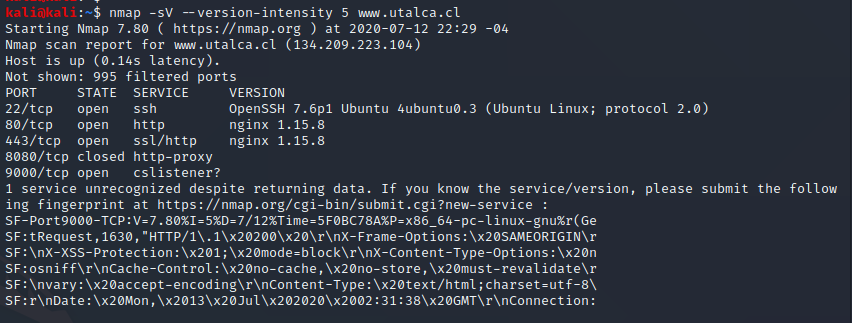
\includegraphics[width=.75\textwidth]{images2/nmap.png}
\end{figure}

El primer análisis entregado por NMAP no es muy alentador. A diferencia de ocasiones anteriores, en este caso al parecer solo están abiertos los puertos para el consumo de tráfico web y un openssh que está protegido con un acceso solo por llave privada (bien jugado, aprendieron).

Adicionalmente hay un puerto abierto, el 9000 que típicamente en estos casos queda abierto para ser utilizado por sentry, lo cual no debería de ser tan sorprendente.


\subsection{Actividad 2 - OWASP ZAP}

\begin{figure}[H]
	\centering
	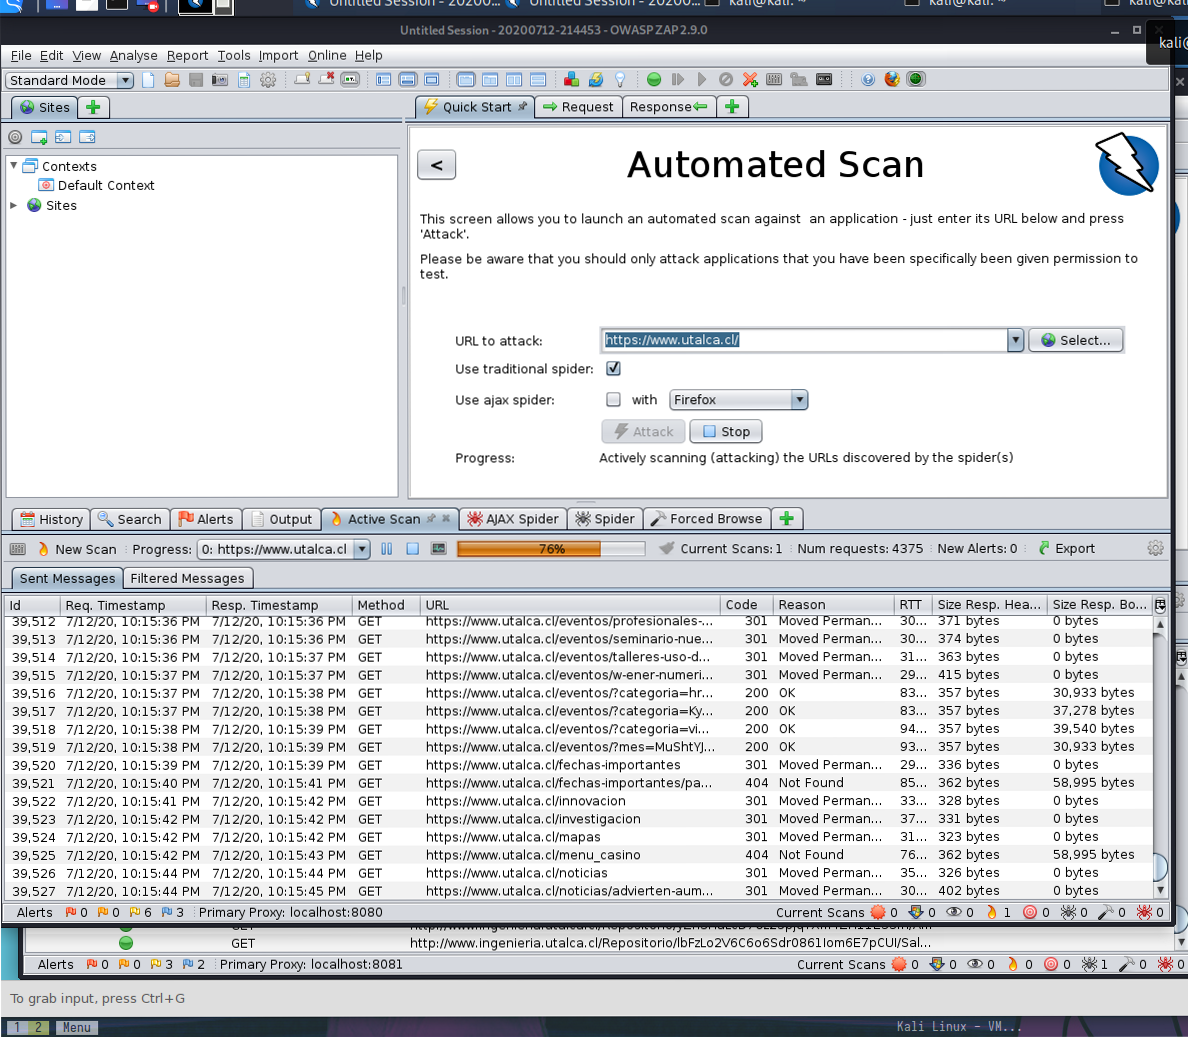
\includegraphics[width=.75\textwidth]{images2/zap1.png}
\end{figure}
Inicio de la ejecución de OWASP ZAP. Utilizamos los parámetros por defecto el cual ejecuta una búsqueda estandar. No hay necesidad de probar otras arañas ya que la diferencia por headers es nula. Durante esta ejecución es posible apreciar dos procesos principales. La araña que se encarga de buscar la información del sitio y realizar un mapa de este y la ejecución activa de los ataques -aka probing-.


\begin{figure}[H]
	\centering
	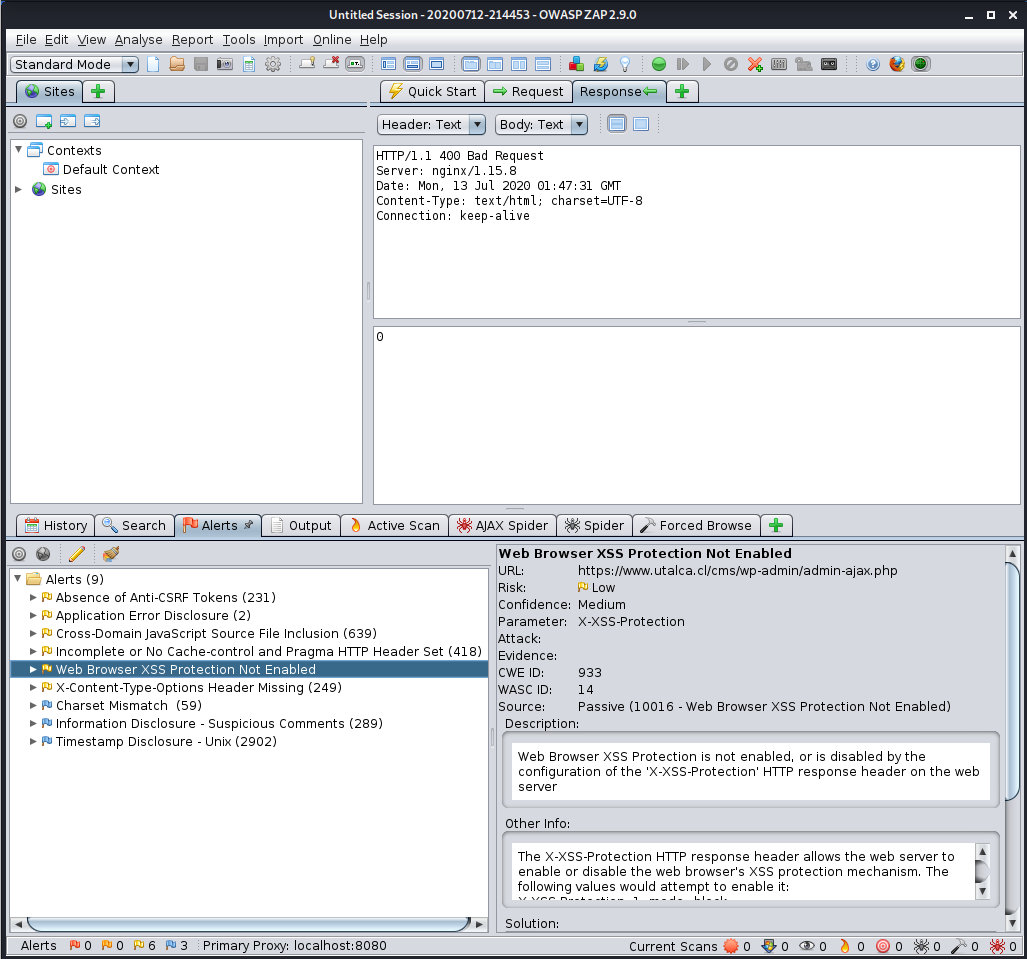
\includegraphics[width=.75\textwidth]{images2/zap2.png}
\end{figure}
Podemos ver una vez terminada la ejecución de ZAP que no se encuentran mayores vulnerabilidades, aunque llama la atención el número de alertas que son lanzadas por la herramienta en si.
\begin{figure}[H]
	\centering
	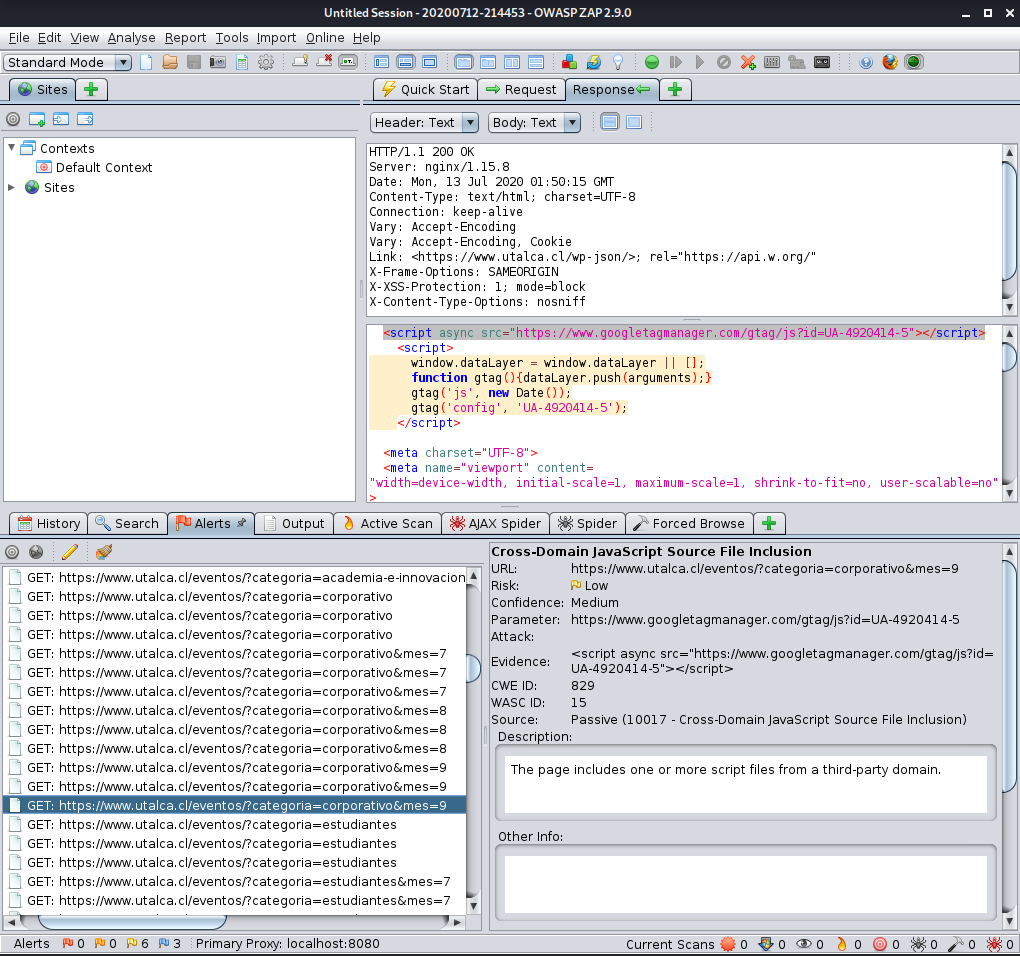
\includegraphics[width=.75\textwidth]{images2/zap4.png}
\end{figure}
En si, la ejecución de ZAP como muchas herramientas automatizadas para la búsqueda de vulnerabilidades es muy propensa a encontrar falsos positivos. Por ejemplo, tomemos este caso de supuesta ejecución remota.

Podemos apreciar que se incluye un archivo desde google tag manager, por lo que si, es un problema el estar incluyendo archivos de una fuente de terceros. Sin embargo, el objetivo de este laboratorio es encontrar vulnerabilidades dentro de la aplicación en si y esta solo afecta al cliente, por ejemplo, cuando este dominio está pasando por un ataque MITM entonces el cliente puede ser afectado al cargar un script diferente. 

Sin embargo, no es un problema propio de la aplicación. De todas maneras, esta información es valiosa al momento de realizar un assesment, ya que nos sugiere que un buen vector de ataque lateral son usuarios que acceden al sitio y poseean credenciales y con los que podamos tener contacto dentro de la misma red.

La existencia de estas URL con parámetros nos sugiere un buen punto de partida para probar inyecciones SQL.

\begin{figure}[H]
	\centering
	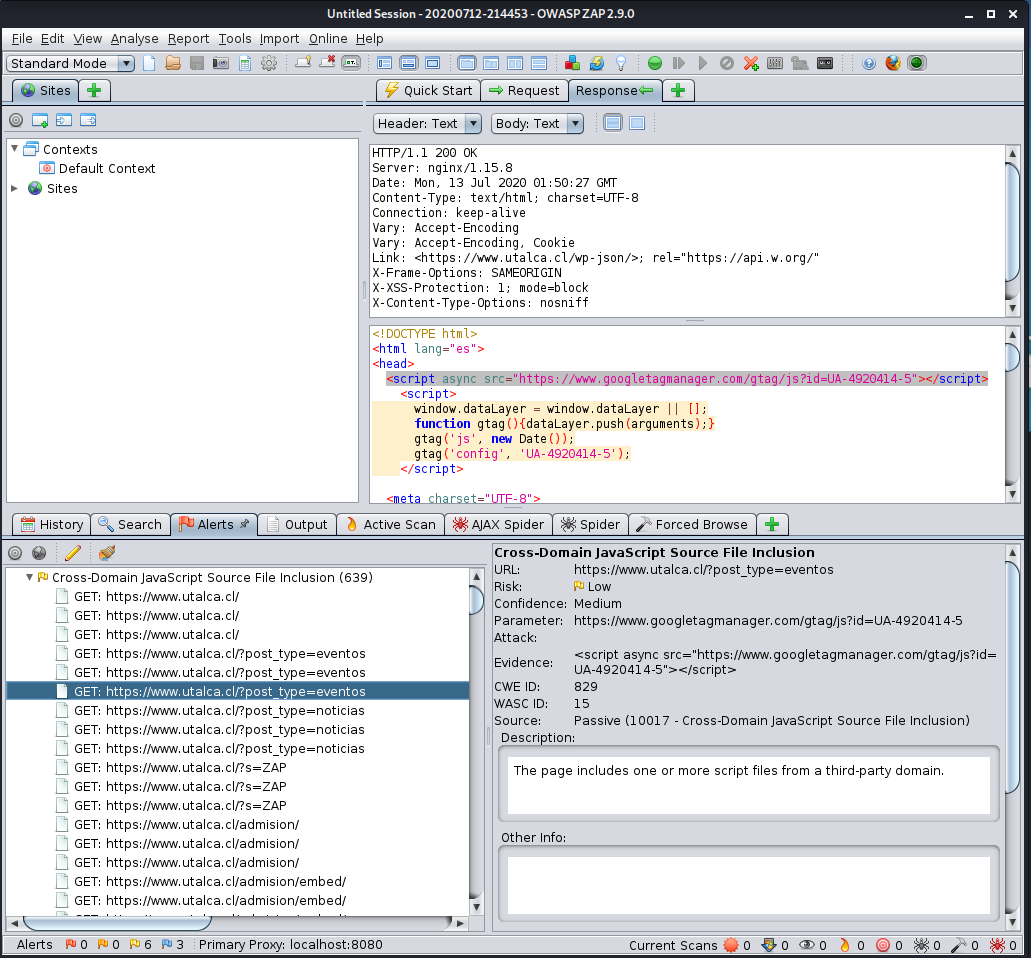
\includegraphics[width=.75\textwidth]{images2/zap3.png}
\end{figure}

Sin embargo, al revisar mas en profundidad las alertas entregadas, además de confirmar los falsos positivos, encontramos que en realidad la razón de la gran cantidad de estos es porque derechamente hay una cantidad enorme de malas prácticas de programación involucradas en el desarrollo del sitio (sin contar que es un wordpress).



\subsection{Actividad 3 - NIKTO}

Para este caso utilizamos el siguiente comando para almacenar la información dentro de un archivo: \texttt{nikto -Display V -o results.html -Format htm -h https://www.utalca.cl}. 


\begin{figure}[H]
	\centering
	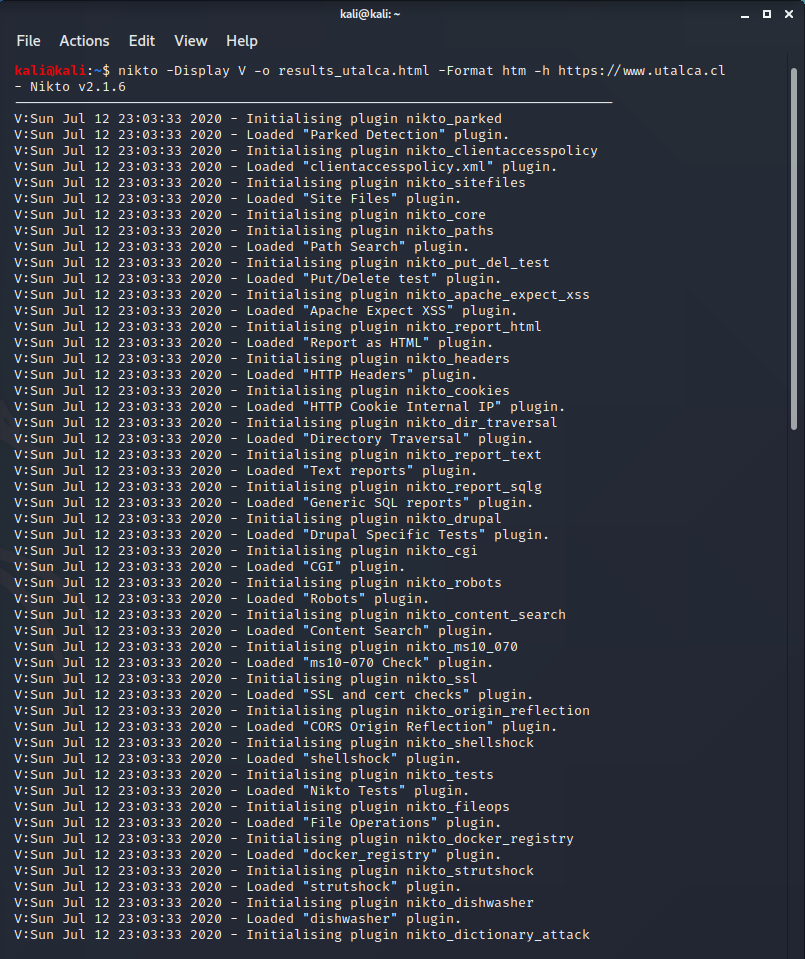
\includegraphics[width=.75\textwidth]{images2/nikto1.png}
\end{figure}


Sin embargo nos topamos con un problema fundamental, sin embargo que nos impide utilizar esta herramienta por completo. Al parecer el servidor tiene tiempos de respuesta relativamente altos para las consultas, no a su vez con la resolución de recursos estáticos. 


\begin{figure}[H]
	\centering
	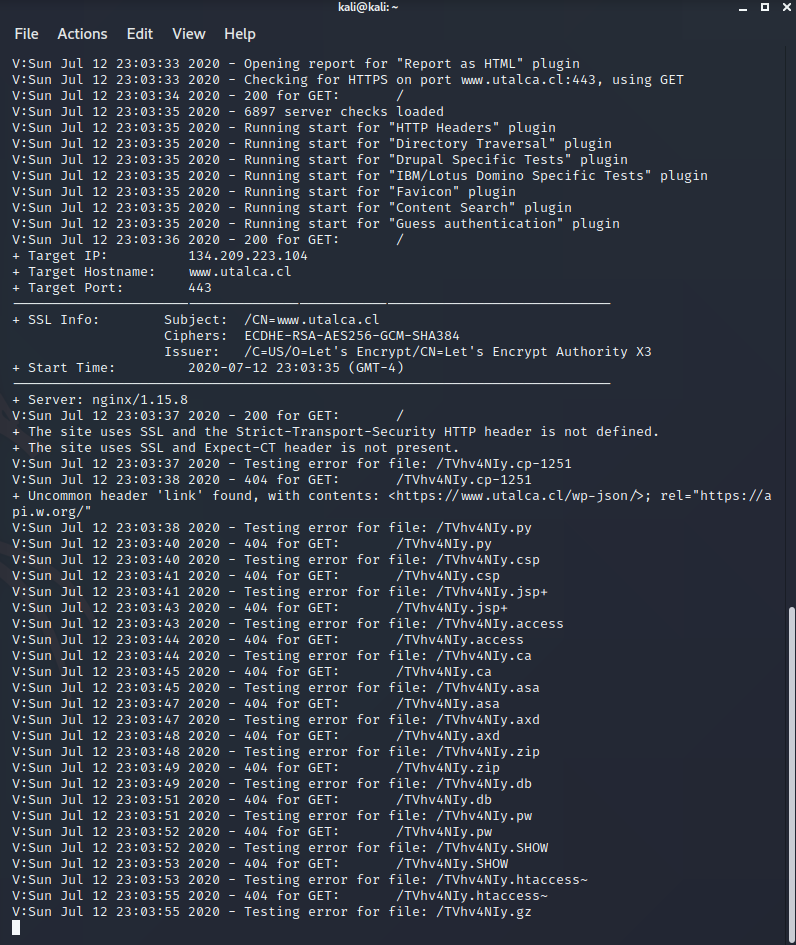
\includegraphics[width=.75\textwidth]{images2/nikto2.png}
\end{figure}

Debido a que NIKTO prueba los ataques de manera secuencial, al momento de ejecutar un ataque para poder revisar los archivos disponibles, tenemos un retraso de aproximadamente 500ms a 1600ms. Hay dos hipótesis al respecto, la primera es que toda esta plataforma está bajo un tarpit, la segunda es que el servidor está bajo mucho estrés o bien está mal configurado. Históricamente se ha probado que es mas probable que sea la segunda opción, sin embargo, este problema nos impide resolver el comando dentro de un tiempo relativamente "razonable". 


\begin{figure}[H]
	\centering
	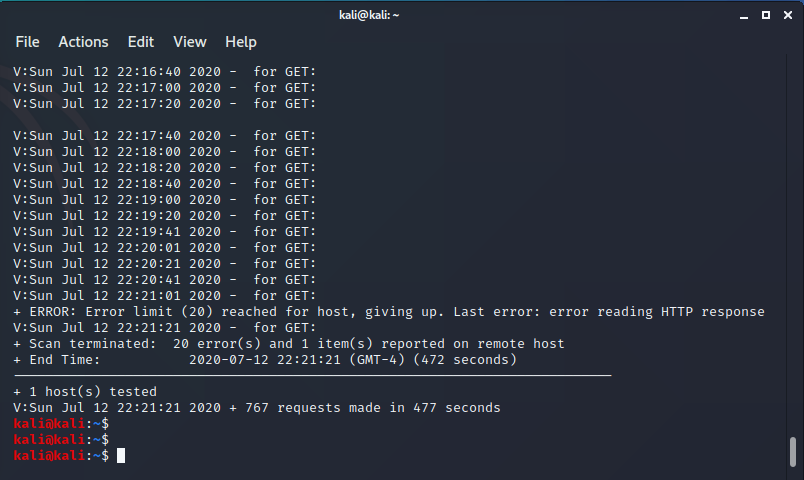
\includegraphics[width=.75\textwidth]{images2/nikto3.png}
\end{figure}

Ahora el problema de esto no es que sea lento el análisis (nikto por naturaleza es lento), si no que el analisis en vez de tomar horas, pasa a tomar días solo por el efecto del tarpit. Incluso paralelizando los análisis, no se obtienen resultados conluyentes ya que no alcanza a realizar todo el trabajo en un tiempo relativamente razonable (digamos, unas 5 horas).



\subsection{Actividad 3 - SQLMAP}
Para efectos de simpleza solo se muestra una ejecución.

\begin{figure}[H]
	\centering
	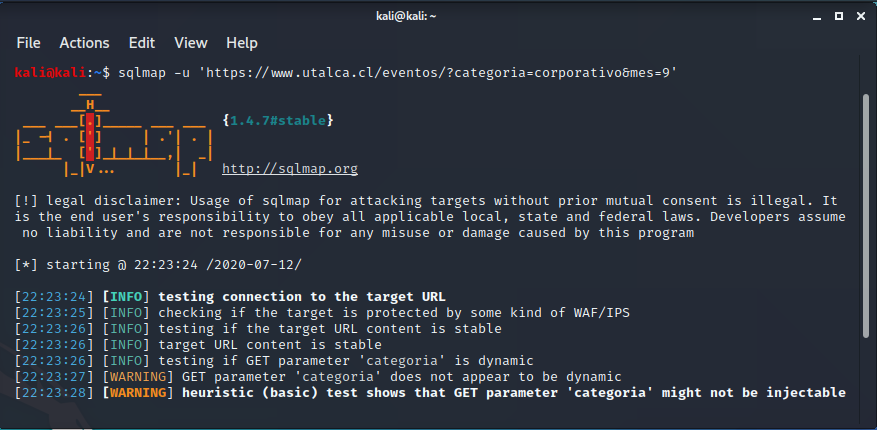
\includegraphics[width=.75\textwidth]{images2/sqlmap1.png}
\end{figure}

Utilizando la url descubierta en el paso anterior (en realidad se probó con un conjunto de estas), procedemos a ejecutar SQLMAP sobre la dirección. Dado que no estamos necesariamente trabajando con scripts de inyección específicos, no utilizamos mayores argumentos.

\begin{figure}[H]
	\centering
	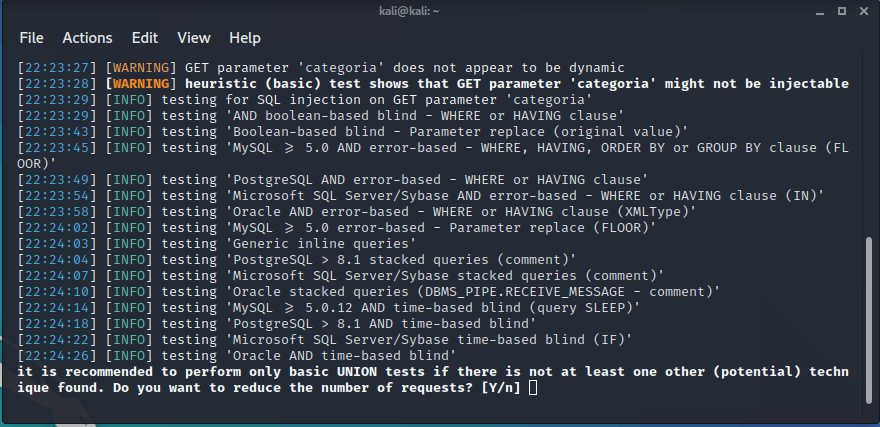
\includegraphics[width=.75\textwidth]{images2/sqlmap2.png}
\end{figure}

Sin embargo en los primeros 10 minutos podemos ver que la ejecución se detiene dentro del modo interactivo indicando que no hay vectores de ataque por inyección por tanto sugiere cambiar la estrategia. A esto se le dice que si y continúa el análisis.

\begin{figure}[H]
	\centering
	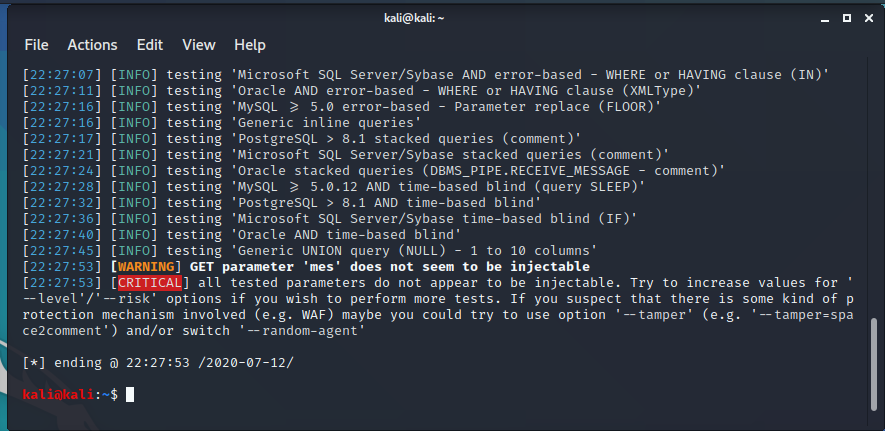
\includegraphics[width=.75\textwidth]{images2/sqlmap3.png}
\end{figure}

Sin embargo al cabo de un tiempo, notamos que no arroja mayores resultados. Esto pasó con todas las URL probadas que salieron de la ejecución de la araña de ZAP.

\section{Conclusiones}
Si bien todas las herramientas fallaron, esto no quiere decir que la aplicación esté libre de fallas. En primer lugar, todos las pruebas fueron ejecutadas desde una máquina en la red, por tanto la situación podría ser diferente al intentarlos dentro de la misma red de la universidad. 

Adicionalmente, como se pudo observar durante la ejecución de ZAP, la aplicación en si cuenta con malas prácticas de programación por parte de los módulos de terceros invlucrados en esta.

De ejecutarse un análisis, este no solo debe hacerse a nivel de la aplicación en si como lo especifica el enunciado, se tiene que tomar en cuenta otros sitios los cuales puedan servir como vectores laterales, sitios relacionados, revisar la estructura de la red y los servicios ya que en este caso, resulta que el sitio en cuestion es simplemente un front-end para otra aplicación conectada por detras.

\begin{thebibliography}{9}

	\bibitem{REF:sqlmap}
	Documentación de sqlmap
	\textit{sqlmap homepage}.
	http://sqlmap.org/

	\bibitem{REF:nmap}
	Documentación de nmap
	\textit{nmap homepage}.
	https://nmap.org/

	\bibitem{REF:OWASP ZAP}
	Documentación de OWASP ZAP
	\textit{OWASP ZAP project homepage}.
	https://owasp.org/www-project-zap/


	\bibitem{REF:nikto}
	RedTeamTutorials
	\textit{NIKTO Cheat Sheet}.
	https://redteamtutorials.com/2018/10/24/nikto-cheatsheet/
\end{thebibliography}

\end{document}